\documentclass{standalone}
\usepackage{tikz}
\usepackage{ctex,siunitx,bm}
\setCJKmainfont{Noto Serif CJK SC}
\usepackage{tkz-euclide,ninecolors}
\usepackage{amsmath}
\usetikzlibrary{patterns, calc}
\usetikzlibrary {decorations.pathmorphing, decorations.pathreplacing, decorations.shapes}
\pgfdeclareverticalshading{pile}{100bp}{
  color(0bp)=(black);color(25bp)=(black);color(50bp)=(white);color(75bp)=(black);color(100bp)=(black)
}
\pgfdeclareverticalshading{pile2}{100bp}{
  color(0bp)=(white);color(50bp)=(black);color(100bp)=(white)
}
\begin{document}
\small
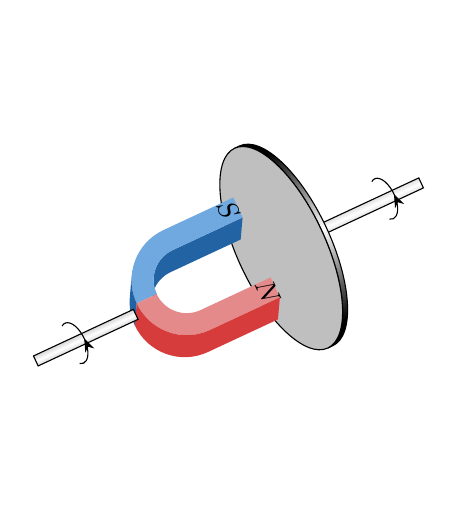
\begin{tikzpicture}[>=latex,scale=1.4]
  \useasboundingbox(-2.3,2.0)rectangle(1.35,-2.1);
  \begin{scope}[rotate=205]
    \draw[shading=pile,shading angle=25](0,-0.05)rectangle++(-1.4,0.1);
    \draw[postaction={decorate},decoration={markings,mark= at position 0.5 with {\arrowreversed{Stealth[scale=1]}}}](-1.0,-0.2)arc(290:70:0.1 and 0.2);
    \draw[shading=pile,shading angle=25](0,1)--(-0.05,1)arc(90:270:0.4 and 1.0)--++(0.05,0)arc(270:90:0.4 and 1.0)--cycle;
    \draw[fill=lightgray](0,0)ellipse(0.4 and 1.0);
    \fill[azure4](0.9,-0.4)--(0.2,-0.4)--++(60:0.2)--++(0.7,0)arc(-90:0:0.3)--++(60:-0.2)arc(0:-90:0.3);
    \fill[azure7](0.2,-0.4)--(0.9,-0.4)arc(-90:0:0.3)--++(0.2,0)arc(0:-90:0.5)--(0.2,-0.6);
    \fill[red7](1.2,-0.1)arc(0:90:0.3)--(0.2,0.2)--(0.2,0.4)--(0.9,0.4)arc(90:0:0.5)--cycle;
    \fill[red5](0.2,0.4)--++(60:0.2)--++(0.7,0)arc(90:0:0.5)--++(240:0.2)arc(0:90:0.5)--cycle;
    \fill[azure4](1.4,-0.1)arc(0:-30:0.5)--++(60:0.2)arc(-30:0:0.5)--cycle;
    \draw[shading=pile,shading angle=25](1.45,-0.0634)rectangle++(1,0.1);
    \draw[postaction={decorate},decoration={markings,mark= at position 0.5 with {\arrowreversed{Stealth[scale=1]}}}](2.1,-0.2)arc(290:70:0.1 and 0.2);
  \end{scope}
  \node at (-0.12,-0.4)[rotate=-65]{$N$};
  \node at (-0.48,0.35)[rotate=-65]{$S$};
\end{tikzpicture}
\end{document}